\documentclass[a4paper,11pt,oneside]{article}

\usepackage[utf8]{inputenc}
\usepackage[a4paper,top=3cm,bottom=3cm,left=3cm,right=3cm]{geometry}
\renewcommand{\familydefault}{\sfdefault}
\usepackage{helvet}
\usepackage[ruled,vlined]{algorithm2e}
\usepackage{amsmath}
\usepackage{amsthm}
\usepackage{csquotes}
\usepackage{tabularx}
\usepackage{array}
\usepackage[english]{babel}     %% typographie française
\usepackage[backend=bibtex,style=numeric,language=english]{biblatex}
\usepackage{parskip}		%% blank lines between paragraphs, no indent
\usepackage[margin=1cm]{caption}%% give long captions a margin
\usepackage{booktabs}           %% typesetting nice tables
\usepackage[pdftex]{graphicx}	%% include graphics, preferrably pdf
\usepackage[pdftex]{hyperref}	%% many PDF options can be set here
\pdfadjustspacing=1		%% force LaTeX-like character spacing

\newenvironment{conditions}
  {\par\vspace{\abovedisplayskip}\noindent\begin{tabular}{>{$}l<{$} @{${}={}$} l}}
  {\end{tabular}\par\vspace{\belowdisplayskip}}

\newcommand{\myname}{Otmane Sabir}
\newcommand{\mytitle}{Constructive Solid Geometry}
\newcommand{\mysupervisor}{Prof. Dr. Sergey Kosov}

\hypersetup{
  pdfauthor = {\myname},
  pdftitle = {\mytitle},
  pdfkeywords = {},
  colorlinks = {true},
  linkcolor = {blue},
  citecolor = {blue}	
}

\addbibresource{references.bib}

\begin{document}
\pagenumbering{roman}

\thispagestyle{empty}

\begin{flushright}
	
\includegraphics[scale=0.8]{bsc-logo}
\end{flushright}
\vspace*{40mm}
\begin{center}
	\huge
	\textbf{\mytitle}
\end{center}
\vspace*{4mm}
\begin{center}
	\Large by
\end{center}
\vspace*{4mm}
\begin{center}
	\LARGE
	\textbf{\myname}
\end{center}
\vspace*{20mm}
\begin{center}
	\Large
	Bachelor Thesis in Computer Science
\end{center}
\vfill
\begin{flushleft}
	\large
	Submission: \today \hfill Supervisor: \mysupervisor \\
	\rule{\textwidth}{1pt}
\end{flushleft}
\begin{center}
	Jacobs University Bremen $|$ Department of Computer Science and Electrical Engineering
\end{center}

\newpage
\thispagestyle{empty}

\subsection*{English: Declaration of Authorship}
 
I hereby declare that the thesis submitted was created and written
solely by myself without any external support. Any sources, direct
or indirect, are marked as such. I am aware of the fact that the
contents of the thesis in digital form may be revised with regard to
usage of unauthorized aid as well as whether the whole or parts of
it may be identified as plagiarism. I do agree my work to be entered
into a database for it to be compared with existing sources, where
it will remain in order to enable further comparisons with future
theses. This does not grant any rights of reproduction and usage,
however.

This document was neither presented to any other examination board
nor has it been published.

\subsection*{German: Erklärung der Autorenschaft (Urheberschaft)}
 
Ich erkläre hiermit, dass die vorliegende Arbeit ohne fremde Hilfe
ausschließlich von mir erstellt und geschrieben worden ist. Jedwede
verwendeten Quellen, direkter oder indirekter Art, sind als solche
kenntlich gemacht worden. Mir ist die Tatsache bewusst, dass der
Inhalt der Thesis in digitaler Form geprüft werden kann im Hinblick
darauf, ob es sich ganz oder in Teilen um ein Plagiat handelt. Ich
bin damit einverstanden, dass meine Arbeit in einer Datenbank
eingegeben werden kann, um mit bereits bestehenden Quellen
verglichen zu werden und dort auch verbleibt, um mit zukünftigen
Arbeiten verglichen werden zu können. Dies berechtigt jedoch nicht
zur Verwendung oder Vervielfältigung.

Diese Arbeit wurde noch keiner anderen Prüfungsbehörde vorgelegt
noch wurde sie bisher veröffentlicht.

\vspace{20mm}

Date, Signature

\newpage

\section*{Abstract}
  
% TODO: add this reference
% http://www.cs.unc.edu/~fuchs/publications/VisSurfaceGeneration80.pdf
   
  
(target size: 15-20 lines)

\newpage
\tableofcontents

\clearpage
\pagenumbering{arabic}

\section{Introduction}
  
Constructive Solid Geometry (CSG) is a method used in computer graphics, computer-aided design, generic modeling languages, and numerous other applications to construct complex geometries from simple primitives or polyhedral solids through the use of boolean operators, namely union ($\cup$),  difference ($\ominus$), and intersection ($\cap$). Figure \ref{fig1:set_operations_examples}a through \ref{fig1:set_operations_examples}c respectively show intersection, union, and difference operations. The approach grows especially appealing when implemented in a ray tracing system as the core intricacy renders performing arithmetic logic on a pair of uni-dimensional rays. Nonetheless, most current ray tracing systems generally suffer from the detriment of the expensive object space intersection computation, and the generic CSG algorithms suffer immensely from their computational complexity, making it very difficult to integrate into operating rendering engines. Therefore, this research concentrates on constructive solid geometry and possible means of acceleration.
  
\begin{figure}[ht]
	\begin{center}
		
\includegraphics[width=.6\textwidth]{intro-figures/figure1.png}
	\end{center}
	\caption{Examples of set operations on a mesh sphere and box.}
	\label{fig1:set_operations_examples}
\end{figure}
  
\subsection{Rendering Algorithms}
  
Rendering digital photorealistic or non-photorealistic images has been a topic of study since the late 1960s \cite{INITIAL_RENDERING}. Since then, various algorithms came forth that allow achieving different results depending on the required conditions. Inherently all these algorithms strive to solve the same underlying problem by trading-off different aspects, namely speed and realism. This problem is known as the hidden surface problem. The hidden surface problem is determining the visible objects in space from a certain point of view. There are two general methods, object-space methods, which try to start from the object space and project the geometries onto the 2D raster, or the image-space ones, which perform the opposite by tracing a ray through each pixel and attempting to locate the closest intersection of that ray with the geometries in the scene. The two methods then give birth to the pair of most famous and widely adopted rendering algorithms: rasterization and ray tracing.
  
\subsubsection{Rasterization}
    
Rasterization has very quickly become the dominant approach for interactive applications because of its initially low computational requirements, its massive adoption in most hardware solutions, and later by the ever-increasing performance of dedicated graphics hardware. The use of local, per-triangle computation makes it well suited for a feed-forward pipeline. However, the rasterization algorithm has many trade-offs. First, the handling of global effects, such as reflections and realistic shading, is intricate, and second, it's also limited to scenes with meshed geometries.
    
\subsubsection{Ray Tracing}
     
Ray tracing simulates the photographic process in reverse. For each pixel on the screen, we shoot a ray and identify objects that intersect the ray. A ray-tracing algorithm makes usage of four essential components: the camera, the geometry, the light sources, and the shaders. These components can have different varieties, to state a few, orthographic and perspective cameras, unidirectional and area light sources, and Phong and chrome shaders. Hence, it allows achieving several outcomes depending on the necessities. The main downside has been computational time and the constraints of using such an algorithm in interactive applications. However, ray tracing parallelizes efficiently and trivially. Thus it takes advantage of the continuously rising computational power of the hardware. Many applications have successfully produced real-time ray tracing algorithms and allow for highly photorealistic results in interactive applications \cite{RT_RT1, RT_RT2}.
    
  
\subsection{Geometric Representations}
\label{sec:geometric_represections}

When it comes to computer graphics, we can find numerous types of geometry descriptions \cite{SOLIDREP_5, SOLIDREP_1, SOLIDREP_2, SOLIDREP_3, COMPUTING_SURVEYS,SOLIDREP_4}. Many solutions exist that enable the simple conversion between these geometric formats \cite{steuer_2012}. However, there are predominantly two different representations in most geometric modeling systems \cite{COMPUTING_SURVEYS}: boundary representations - commonly known as B-Rep or BREP - and constructive solid geometry - CSG. Each one of these representations brings forward different advantages, disadvantages, and limitations.
    
\subsubsection{Boundary Representation}
    
Boundary representations are indirect definitions of solids in space using their boundary or limit. This representation is usually a hierarchical composition of different dimensionally complex parts. On the very top, we have definitions of two-dimensional faces, which build on uni-dimensional edges that are subsequently built on dimensionless points (See figure \ref{fig2:brep_3d_rect}). A BREP with non-curvilinear edges and planar faces is called a polygon mesh. The points representing the edges shared by a single face must always be co-planar. A triangle is the simplest polygon and has the excellent property of always being co-planar. Additionally, polygons of any complexity are representable by a set of triangles. These qualities make triangular meshes a fundamental component in BREPs. The representations built on triangles are also highly optimized for fast operations. Therefore, we will mainly deal with triangular meshes in OpenRT, though it does offer descriptions for tetragon (quadrilateral) meshes.
    
    
\begin{figure}[ht]
	\begin{center}
		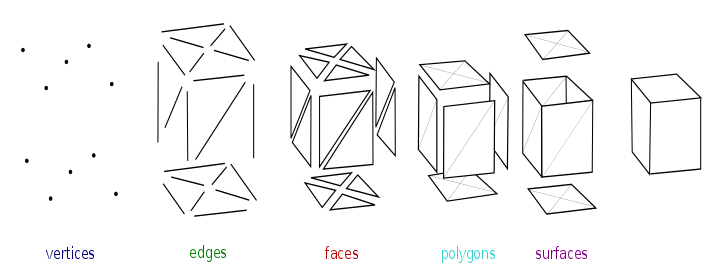
\includegraphics[width=.6\textwidth]{intro-figures/brep-overview.png}
	\end{center}
	\caption{Sample BREP of a 3D hyper-rectangle \cite{wikipedia_2021_mesh_rep}}
	\label{fig2:brep_3d_rect}
\end{figure}
    
\subsubsection{Constructive Solid Geometry}

Constructive solid geometry takes basis on the fundamental premise that any complex physical object is obtainable from a set of primitive geometries and the base boolean operations. CSG is radically different from BREPs as it does not collect any topological information but instead evaluates the geometries as needed by the case scenario. In other words, there is no explicit description of the boundary of the solid. Contrary to BREPs,  CSG representations are quickly modified and manipulated since incremental changes do not trigger re-computation and evaluation of the boundary of a geometry. Therefore, no topological changes occur when adjusting the geometries. The latter makes it an attractive solution as it provides a high-level specification of the objects in space and permits significantly more straightforward modification and manipulation. In the general constructive solid geometry description, the solids are put in a binary tree, referred to as the CSG tree, as Figure \ref{fig3:sample_csg_tree} shows. The root node is the complete composite geometry. The leaf nodes depict the base geometries (cubes, spheres, cylinders, tori, cones, and polygon meshes) used in the composition. Every node in the tree, besides the leaf nodes, expresses another complete solid and contains information of the set operation of that node.
    
\begin{figure}[ht]
	\begin{center}
		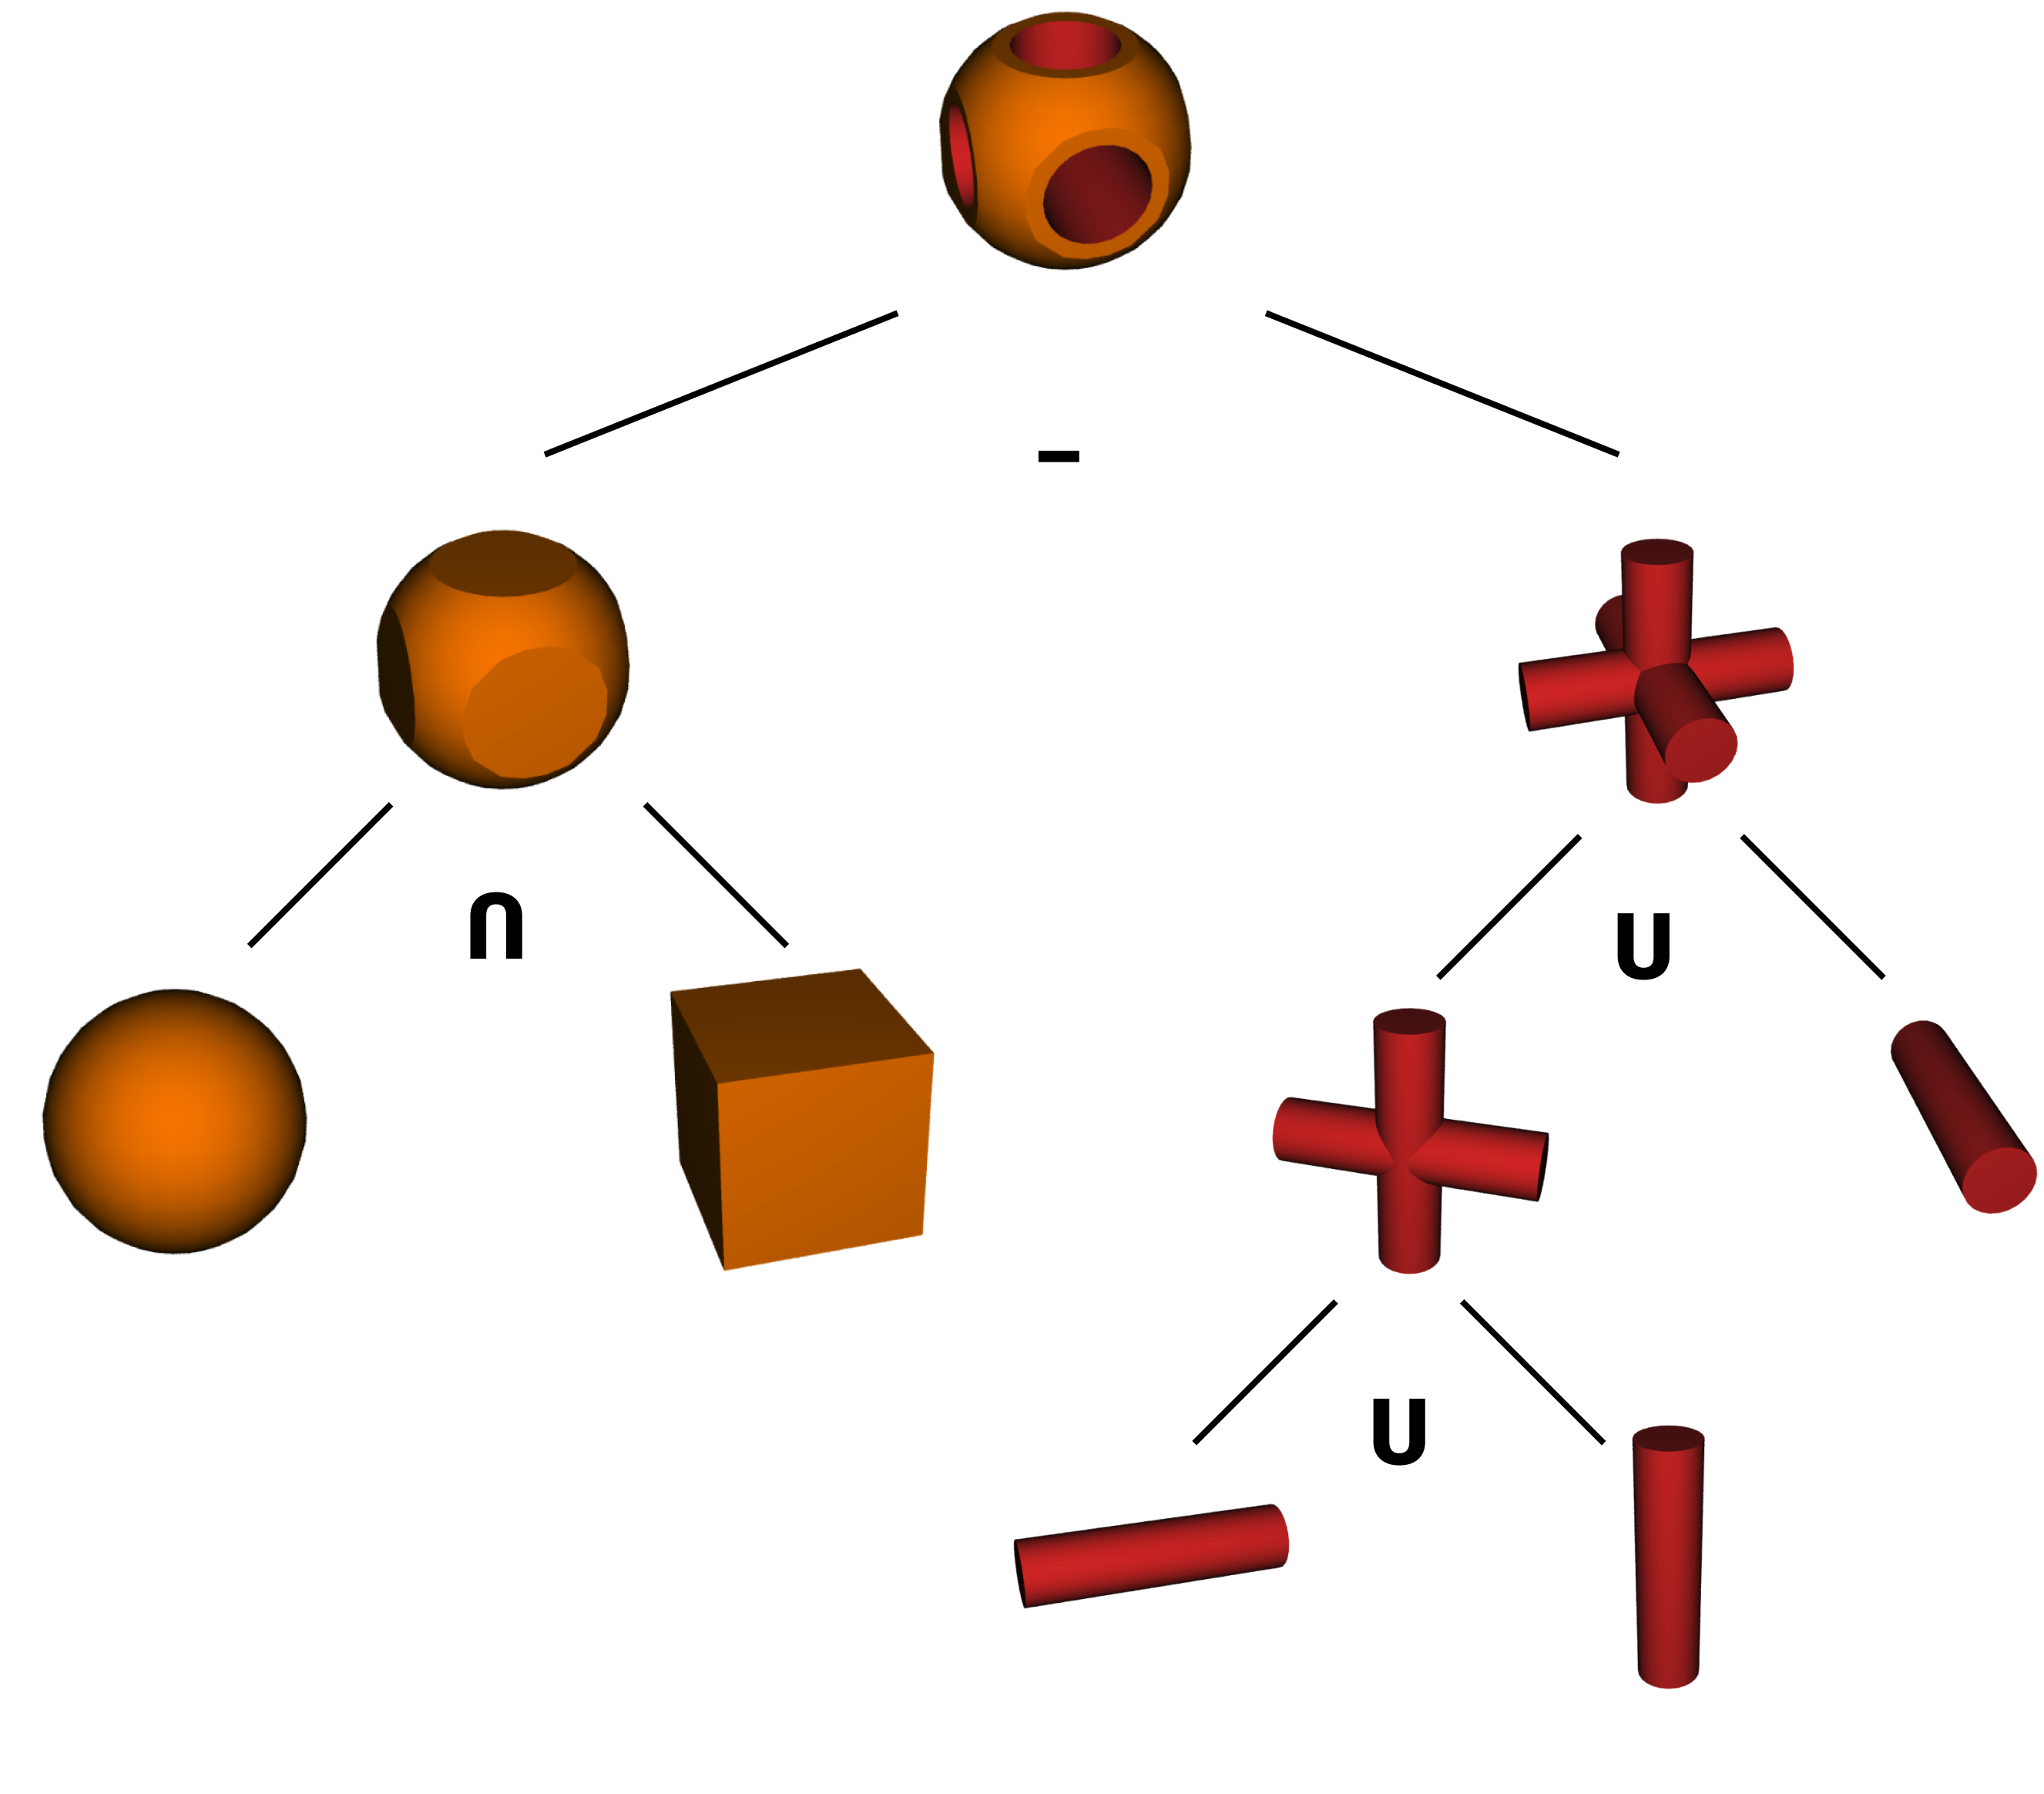
\includegraphics[width=.8\textwidth]{intro-figures/figure3.png}
	\end{center}
	\caption{Basic CSG Tree}
	\label{fig3:sample_csg_tree}
\end{figure}
  
In the OpenRT library implementation, we follow a different approach to allow the use of BREPs as leaf nodes. This gives the flexibility of creating more complex geometries and allowing for nesting of combinatorial geometries inside each other. In a naive implementation, this operation is very costly; however, by using certain spatial indexing structures, each node can be represented as a binary space partitioning tree (See figure \ref{fig4:sample_bsp_tree}).
  
\begin{figure}[ht]
	\begin{center}
		
\includegraphics[width=0.8\textwidth]{intro-figures/figure4.png}
	\end{center}
	\caption{Sample representation of a binary space partitioning (BSP) tree.}
	\label{fig4:sample_bsp_tree}
\end{figure}
  
\subsection{Overview}
  
Following this introduction, we present this CSG implementation in five sections. 2. Related Works; 3. Constructive Solid Geometry; 4. Optimization; 5. Evaluation of the results; 6. Extensions \& Conclusions.
  
The second section presents works already done, the limitations of the proposed implementations, and solutions to problems related to CSG.
  
Section 3 defines the algorithm that performs the logic in the ray-tracing framework. Additionally, we introduce the data structure used to store the needed data for performing the operation, allowing transformations, and finally rendering. Additionally, we present the architecture used to enable the acceleration.
  
Section 4 discusses efficiency and optimizations. The visible surface problem in ray tracing requires a lot of CPU time, and without any optimizations, the CSG algorithm significantly increases the CPU pressure. Therefore, optimizations are much needed to make this method usable and suitable for real-life applications. The speed is a function of the screen resolution and the geometry complexity (how many primitives are in the solid, and the number of nested geometries).
  
Section 5 describes the results received from running various tests on the 3 different implementations of the algorithm. The first is the naive implementation which we refer to as NaiCSG. The second is a variant that uses a Binary Space Partition tree to solve the visible surface problem but still naively finds intersections inside the combinatorial geometry, which we will refer to as BinCSG. Lastly, we'll introduce our optimized algorithm which uses a binary space partition tree on the outside (solving the visible surface problem) and also inside each composite geometry to direct the rays towards the correct geometries, which we will refer to as OptiCSG. We conduct three types tests. The primary one is a function of time and complexity of the geometry, as we monitor the rendering time following gradual increases in the detail level of two sphere meshes. The second computes the time taken to render a scene after covering different amounts of the view port. The third computes the time variations after increasing the number of nested geometries present in the composite solid.
  
  
\section{Related Works}
  
We discuss below the techniques most related to ours. However, there is a tremendous body of work in this area and we; therefore, cannot possibly provide an absolute overview. Our goal is instead to outline similarities and differences with some of the widely adopted approaches for CSG modeling.

Constructive solid geometry has been a subject of study since the late 1970s. It was initially introduced in \cite{GEOMETRIC_MODELING_1977} as a digital solution to help in the design and production activities in the discrete goods industry, this marked the basis for formalizing the method.
  
A rigorous mathematical foundation of constructive solid geometry was later laid out in \cite{Requicha1978MathematicalFO}. The membership classification function, a generalization of the ray clipping method used in CSG, is also thoroughly discussed and various formal properties are introduced.
  
A few years later it was revisited in \cite{ROTH1982109} where \citeauthor{ROTH1982109} et al. (\citeyear{ROTH1982109}) introduced ray casting as a basis for CAD solid modeling systems. Challenges of adequacy and efficiency of ray casting are addressed, and fast picture methods for interactive modeling are introduced to meet the challenges.
  
The focus then turned towards different optimizations of CSG algorithms in the setting of ray tracing. A simplistic and more elegant single hit intersection algorithm is introduced in \cite{kensler_ray_2006}. This suggested mechanism reduces memory load and the number of computations performed to perform ray classification. Though limitations have to be respected since sub-objects must closed, non-self-intersecting, and have consistently oriented normals.
  
A "slicing" approach is also proposed in \cite{lefebvre:hal-00926861}. Similar to our proposed solution combinations of meshes and analytical primitives through CSG operations are permissible. Nevertheless, this approach requires one boolean per primitive and a complete evaluation of the CSG expression; therefore, making it simple but limited, and much better approaches are imaginable.

Bound definitions are also a popular way of significantly reducing the time required by CSG algorithms. If the ray and the geometric entities are bound, we perform one first test to see if the ray and the box around a geometric entity overlap. Only if the boxes overlap does one continue to test to determine whether the ray and the entity overlap. A submitted S-bounds algorithm is brought forth in \cite{bounding_algorithms} as a means of acceleration in the solid modeling and CSG.
  
Techniques that optimize various CSG rendering algorithms, namely the Goldfeather and the layered Goldfeather algorithm, and the Sequenced-Convex- Subtraction (SCS) algorithm are advanced in \cite{hardware_accelerated_image_based_csg.}. Although the work represents a significant improvement towards real-time image-based CSG rendering for complex models,  the main focus is on hardware acceleration.
  

\section{Constructive Solid Geometry}
    
\subsection{Ray Intersection}
\label{section:ray-intersection}

Ray intersection is the essence of all ray tracing systems. We supply the system a ray as input and obtain knowledge on how the ray intersects solids in the scene as an output. In ray casting engines, one only necessitates computing the nearest intersection to assess the given scene. However, when evaluating CSG models, we require both the closest and furthest intersections to arrange the ray intersections. With knowledge of all the information in the scene - essentially the camera model and the solids - an evaluation of the closest and most distant intersection is executed with each returning the latter information:

\begin{conditions}
	\vec{o}     &  is the origin of the ray (i.e: origin of the camera model). \\
	\vec{d}     &  is the direction of the ray (i.e: direction from camera origin to pixel in screen). \\
	t     &  the distance to either the closest or furthest intersection. \\
	prim    &  a pointer holding surface information of the intersected primitive. 
\end{conditions}

We can distinguish two types of ray intersections. Firstly, ray-primitive intersection tests on convex primitives such as blocks, cylinders, cones, spheres. Because the primitives are analytically defined, the solution is solving the analytic intersection equation. Consequently, this means that the intersection solution is primitive-specific. Many resources providing the analytical solutions are available \cite{ray_primitive_intersections}.
Second, we encounter the more generic solid-primitive intersection. As we have previously defined in the introduction, a solid is often a boundary representation composed of several triangles. Hence, the main intricacy in ray-solid intersection renders iterating over all primitives and reducing the problem to ray-primitive intersection tests such that the primitives are triangles - polyhedra more abstractly.
We can consider the ray-solid intersection as a more general form of ray-primitive intersection since a primitive is always representable as a solid bearing a single surface. The interesting consequence of such an abstraction is that if we fire a ray in the scene, the computation for determining ray intersection is:

\begin{algorithm}[H]
	\SetAlgoLined
	\KwResult{$[in, out]$ intersection range}
	initialization\;
	\For{every primitive in the solid}{	
		solve the ray-primitive equations\;
		\uIf{intersection exists}{
			\uIf{current intersection is closer than in}{
				set in to current intersection;
			}
			\uIf{current intersection is further than out}{
				set out to current intersection;
			}
		}
	}
	\caption{Ray-solid furthest and closest intersection.}
\end{algorithm}

The ray-solid intersection test has four possible outcomes (also see Figure \ref{sec3.2:fig1}):
\begin{enumerate}
	\item The ray misses the solid.
	\item The ray is tangent to the solid.
	\item The ray enters and exists the solid.
	\item The ray is inside/on the face of a solid and has one intersection.
\end{enumerate}

\begin{figure}[ht]
	\begin{center}
		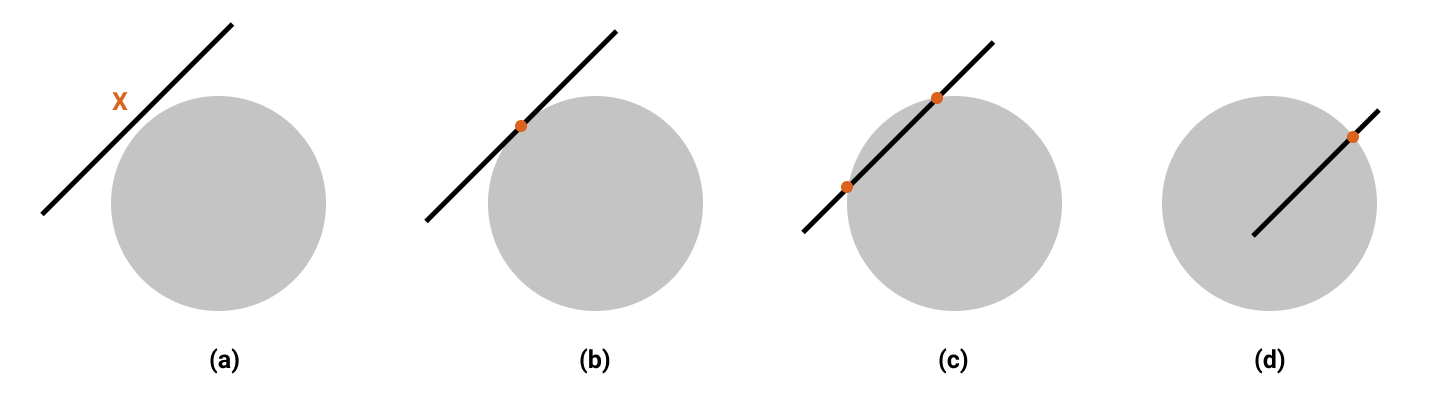
\includegraphics[width=0.8\textwidth]{section3/3.2/intersection_cases.png}
	\end{center}
	\caption{Different ray intersection cases shown on a disk.}
	\label{sec3.2:fig2}
\end{figure}


The first case is self-evident. The second case is also considered as a no intersection result. In case 3, we compute both the entering and exiting points. Case 4 is more interesting as we automatically consider the intersection as "double in", this has some interesting implications which will be discussed in Section 3.4. Since we can now retrieve both $[in, out]$ ray-solid intersection, see figure \ref{sec3.2:fig1}, we can move to the second essential part of our CSG evaluation.

\begin{figure}[ht]
	\begin{center}
		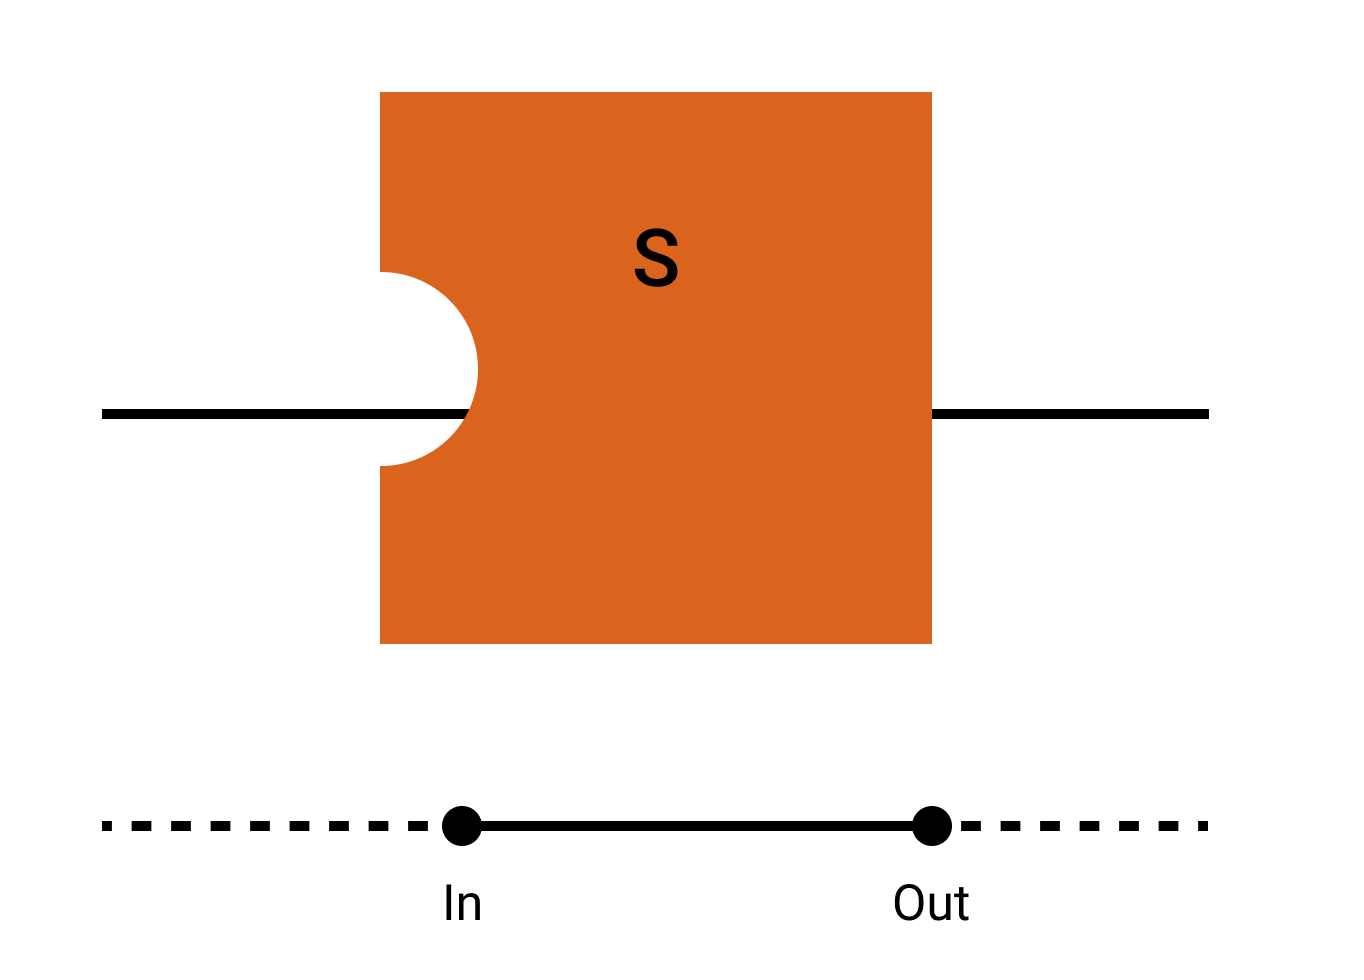
\includegraphics[width=0.4\textwidth]{section3/3.2/ray_intersection.png}
	\end{center}
	\caption{Ray intersection of a solid $S$ with a ray. Where in and out represent the intersection points of this solid.}
	\label{sec3.2:fig1}
\end{figure}

\subsection{Mathematical Formulations}
  
We will be treating a few mathematical formulations as one cannot design a reliable geometric algorithm in the absence of a clear mathematical statement of the problem to be solved. Topology and set theory have been intensively discussed previously in \cite{Requicha1978MathematicalFO}, \cite{tilove1977a}, and other textbooks \cite{lachlan_srebrny_zarach_1977}. Therefore, we will be mainly focusing on definitions and properties that interest us. Formal proofs of the introduced properties are also available in the before-mentioned resources. Constructive solid geometry is based largely on modern Euclidean geometry and the general topology of subsets of three-dimensional Euclidean space $E^3$.
  
\subsubsection{Set Algebra}
  
\theoremstyle{definition}
\newtheorem{definition}{Definition}[section]
  
\theoremstyle{property}
\newtheorem{property}{Property}[section]
    
\theoremstyle{remark}
\newtheorem*{remark}{Remark}
      
\begin{definition}[Set Operations]
	Assume that $X$ and $Y$ are subsets of a universe $W$. We can use the following standard notations:
	      
	\begin{equation} \label{eq:union}
		X \cup Y
	\end{equation}
	\begin{equation} \label{eq:intersection}
		X \cap Y
	\end{equation}
	\begin{equation} \label{eq:difference}
		X \ominus Y
	\end{equation}
	        
	Where \eqref{eq:union}, \eqref{eq:intersection}, and \eqref{eq:difference} denote the union, intersection, and difference of the subsets $X$     and $Y$ respectively. \cite{mansfield_1987}
	        
\end{definition}

\begin{property}
	\label{prop:3.1}
	Union and intersection operations are commutative. \cite{mansfield_1987}
	\begin{equation*}
		X \cup Y = Y \cup X
	\end{equation*}
	\begin{equation*}
		X \cap Y = Y \cap X
	\end{equation*}
\end{property}
        
\begin{property}
	\label{prop:3.2}
	Union and intersection operations are distributive over themselves and each other. \cite{mansfield_1987}
	\begin{equation*}
		X \cup (Y \cap Z) = (X \cup Y) \cap (X \cup Z)
	\end{equation*}
	\begin{equation*}
		X \cap (Y \cup Z) = (X \cap Y) \cup (X \cap Z)
	\end{equation*}
\end{property}
        
\begin{property}
	\label{prop:3.3}
	The empty set $\emptyset$ and the universe $W$ are identity elements for the union and intersection operators. \cite{mansfield_1987}
	\begin{equation*}
		X \cup \emptyset = X
	\end{equation*}
	\begin{equation*}
		X \cap W = X
	\end{equation*}
\end{property}
        
\begin{property}
	\label{prop:3.4}
	The complement, denoted $c$, satisfies \cite{mansfield_1987}:
	\begin{equation*}	
		X \cup cX = W
	\end{equation*}
	\begin{equation*}
		X \cap cX = \emptyset
	\end{equation*}
	\cite{mansfield_1987}
\end{property}


    
\begin{definition}
	A set of elements from the universe $W$ plus the three operators $\cup$, $\cap$, and $\ominus$ that satisfy the properties \eqref{prop:3.1} to \eqref{prop:3.4} is called boolean algebra \cite{Requicha1978MathematicalFO}.
\end{definition}
    
\subsubsection{Topological Spaces}
    
Topological spaces are a generalization of metric spaces in which the notion of "nearness" is introduced but not in any quantifiable way that requires a direct distance definition.
    
\begin{definition}[Topological Space]
	A topological space is a pair $(W, T)$ where $W$ is a set and $T$ is a class of subsets of $W$ called the open sets and satisfying the following three properties:
	\begin{property}
		\label{ts:3.5}
		The empty set $\emptyset$ and the universe $W$ are open.\cite{mansfield_1987}
	\end{property}
	\begin{property}
		\label{ts:3.6}
		The intersection of a finite number of open sets is an open set. \cite{mansfield_1987}
	\end{property}
	\begin{property}
		\label{ts:3.7}
		The union of any collection of open sets is an open set. \cite{mansfield_1987}
	\end{property}
\end{definition}
    
\begin{figure}[ht]
	\begin{center}
		
\includegraphics[width=0.8\textwidth]{section3/3.1/open.png}
	\end{center}
	\caption{A representation of different open sets of varying dimensional order.}
	\label{sect3:open_sets}
\end{figure}
    
\subsubsection{Closed Sets}
\begin{definition}[Closed Sets]
	A subset $X$ of a topological space $(W, T)$ is closed if its complement is open. However, this don't mean that closed sets are the opposite of open sets (e.g. the universe $W$ and the null set $\emptyset$ are both open and closed). Closed sets hold the following properties which are duals of properties \eqref{ts:3.5} to \eqref{ts:3.7}.
		    
	\begin{property}
		The empty set $\emptyset$ and the universe $W$ are closed. \cite{mansfield_1987}
	\end{property}
	\begin{property}
		The union of a finite number of closed sets is a closed set. \cite{mansfield_1987}
	\end{property}
	\begin{property}
		The union of a finite number of closed sets is a closed set. \cite{mansfield_1987}
	\end{property}
\end{definition}
    
\begin{figure}[ht]
	\begin{center}
		
\includegraphics[width=0.8\textwidth]{section3/3.1/closed.png}
	\end{center}
	\caption{A representation of different closed sets of varying dimensional order.}
	\label{sect3:closed_sets}
\end{figure}
    
\subsubsection{Interior}
     
\begin{definition}
	A point of $x$ of $W$ is an interior point of a subset $X$ of $W$ if $X$ is a neighborhood of $x$. The interior of a subset $X$ of $W$, denoted $iX$, is the set of all the interior points of $X$. \cite{Requicha1978MathematicalFO}
\end{definition}
     
\begin{figure}[ht]
	\begin{center}
		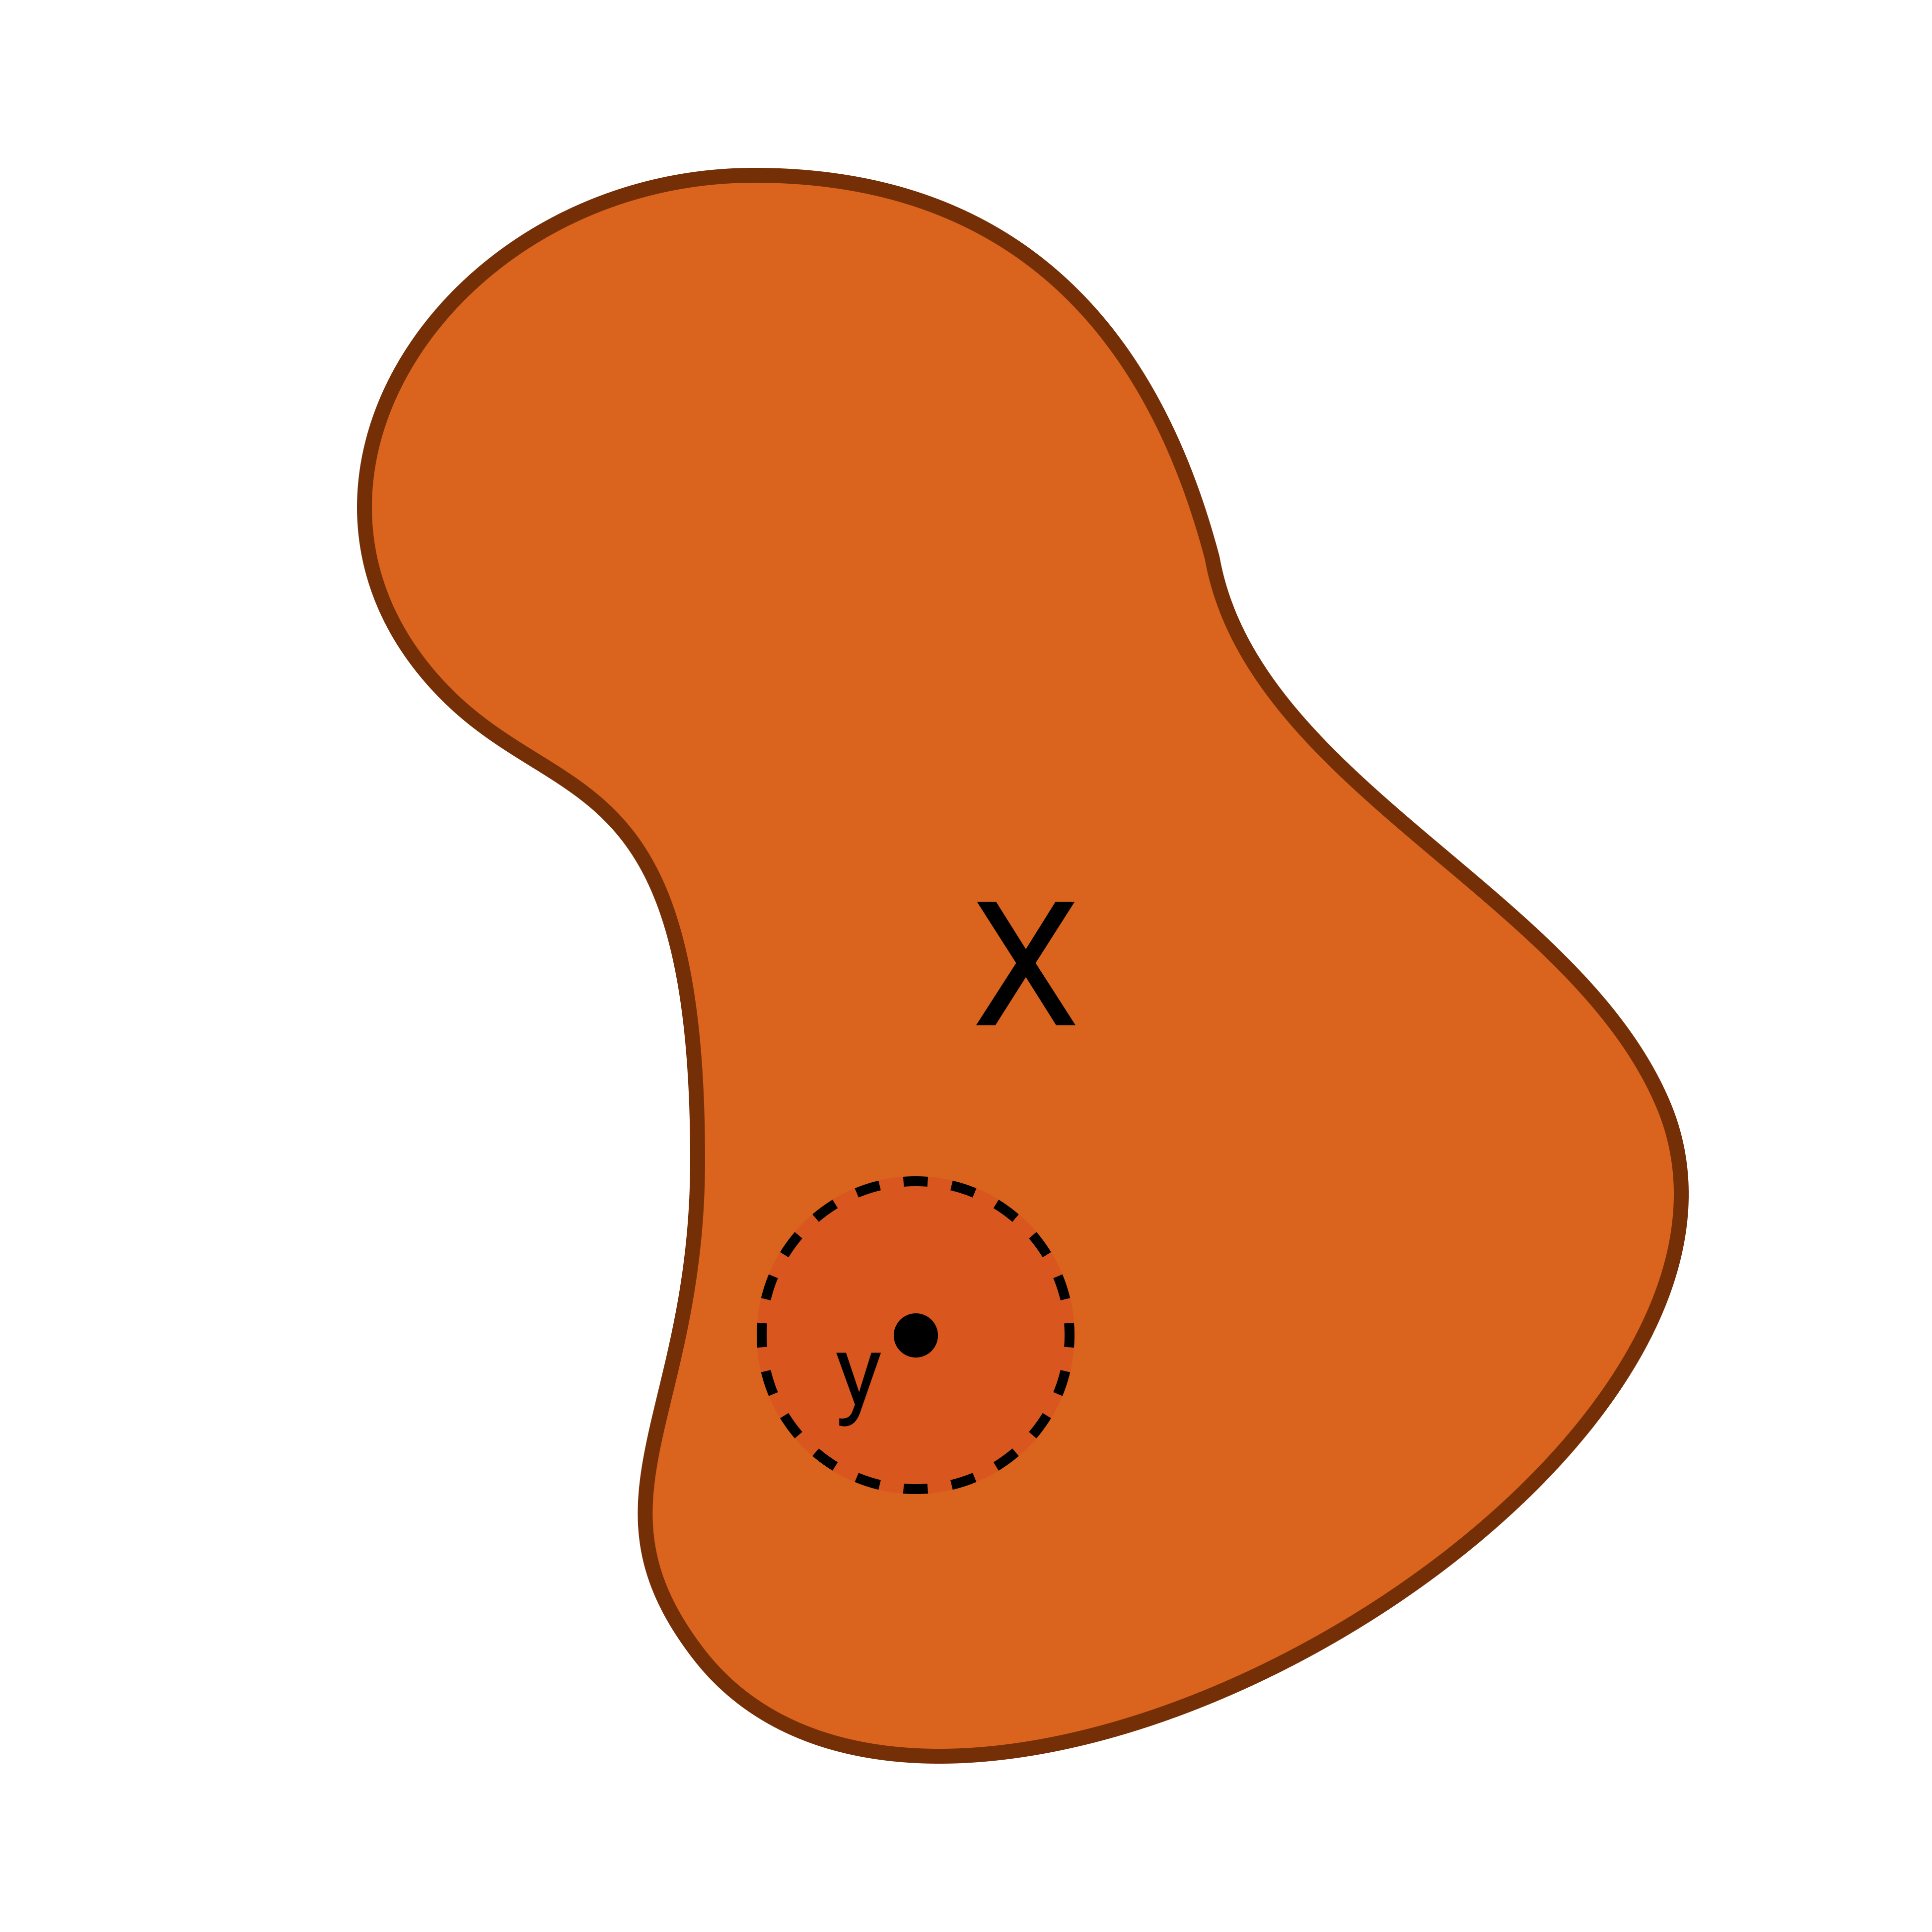
\includegraphics[width=0.3\textwidth]{section3/3.1/interior.png}
	\end{center}
	\caption{Interior point $y$ on a subset $X$.}
	\label{sect3:interior}
\end{figure}
    
\subsubsection{Boundary}
    
\begin{definition}
	A point $x$ of $W$ is a boundary point of a subset $X$ of $W$ if each neighborhood of $x$ intersects both $X$ and $cX$. The boundary of $X$, denoted $bX$, is the set of all boundary points of $X$. \cite{Requicha1978MathematicalFO}
\end{definition}
    
\begin{figure}[ht]
	\begin{center}
		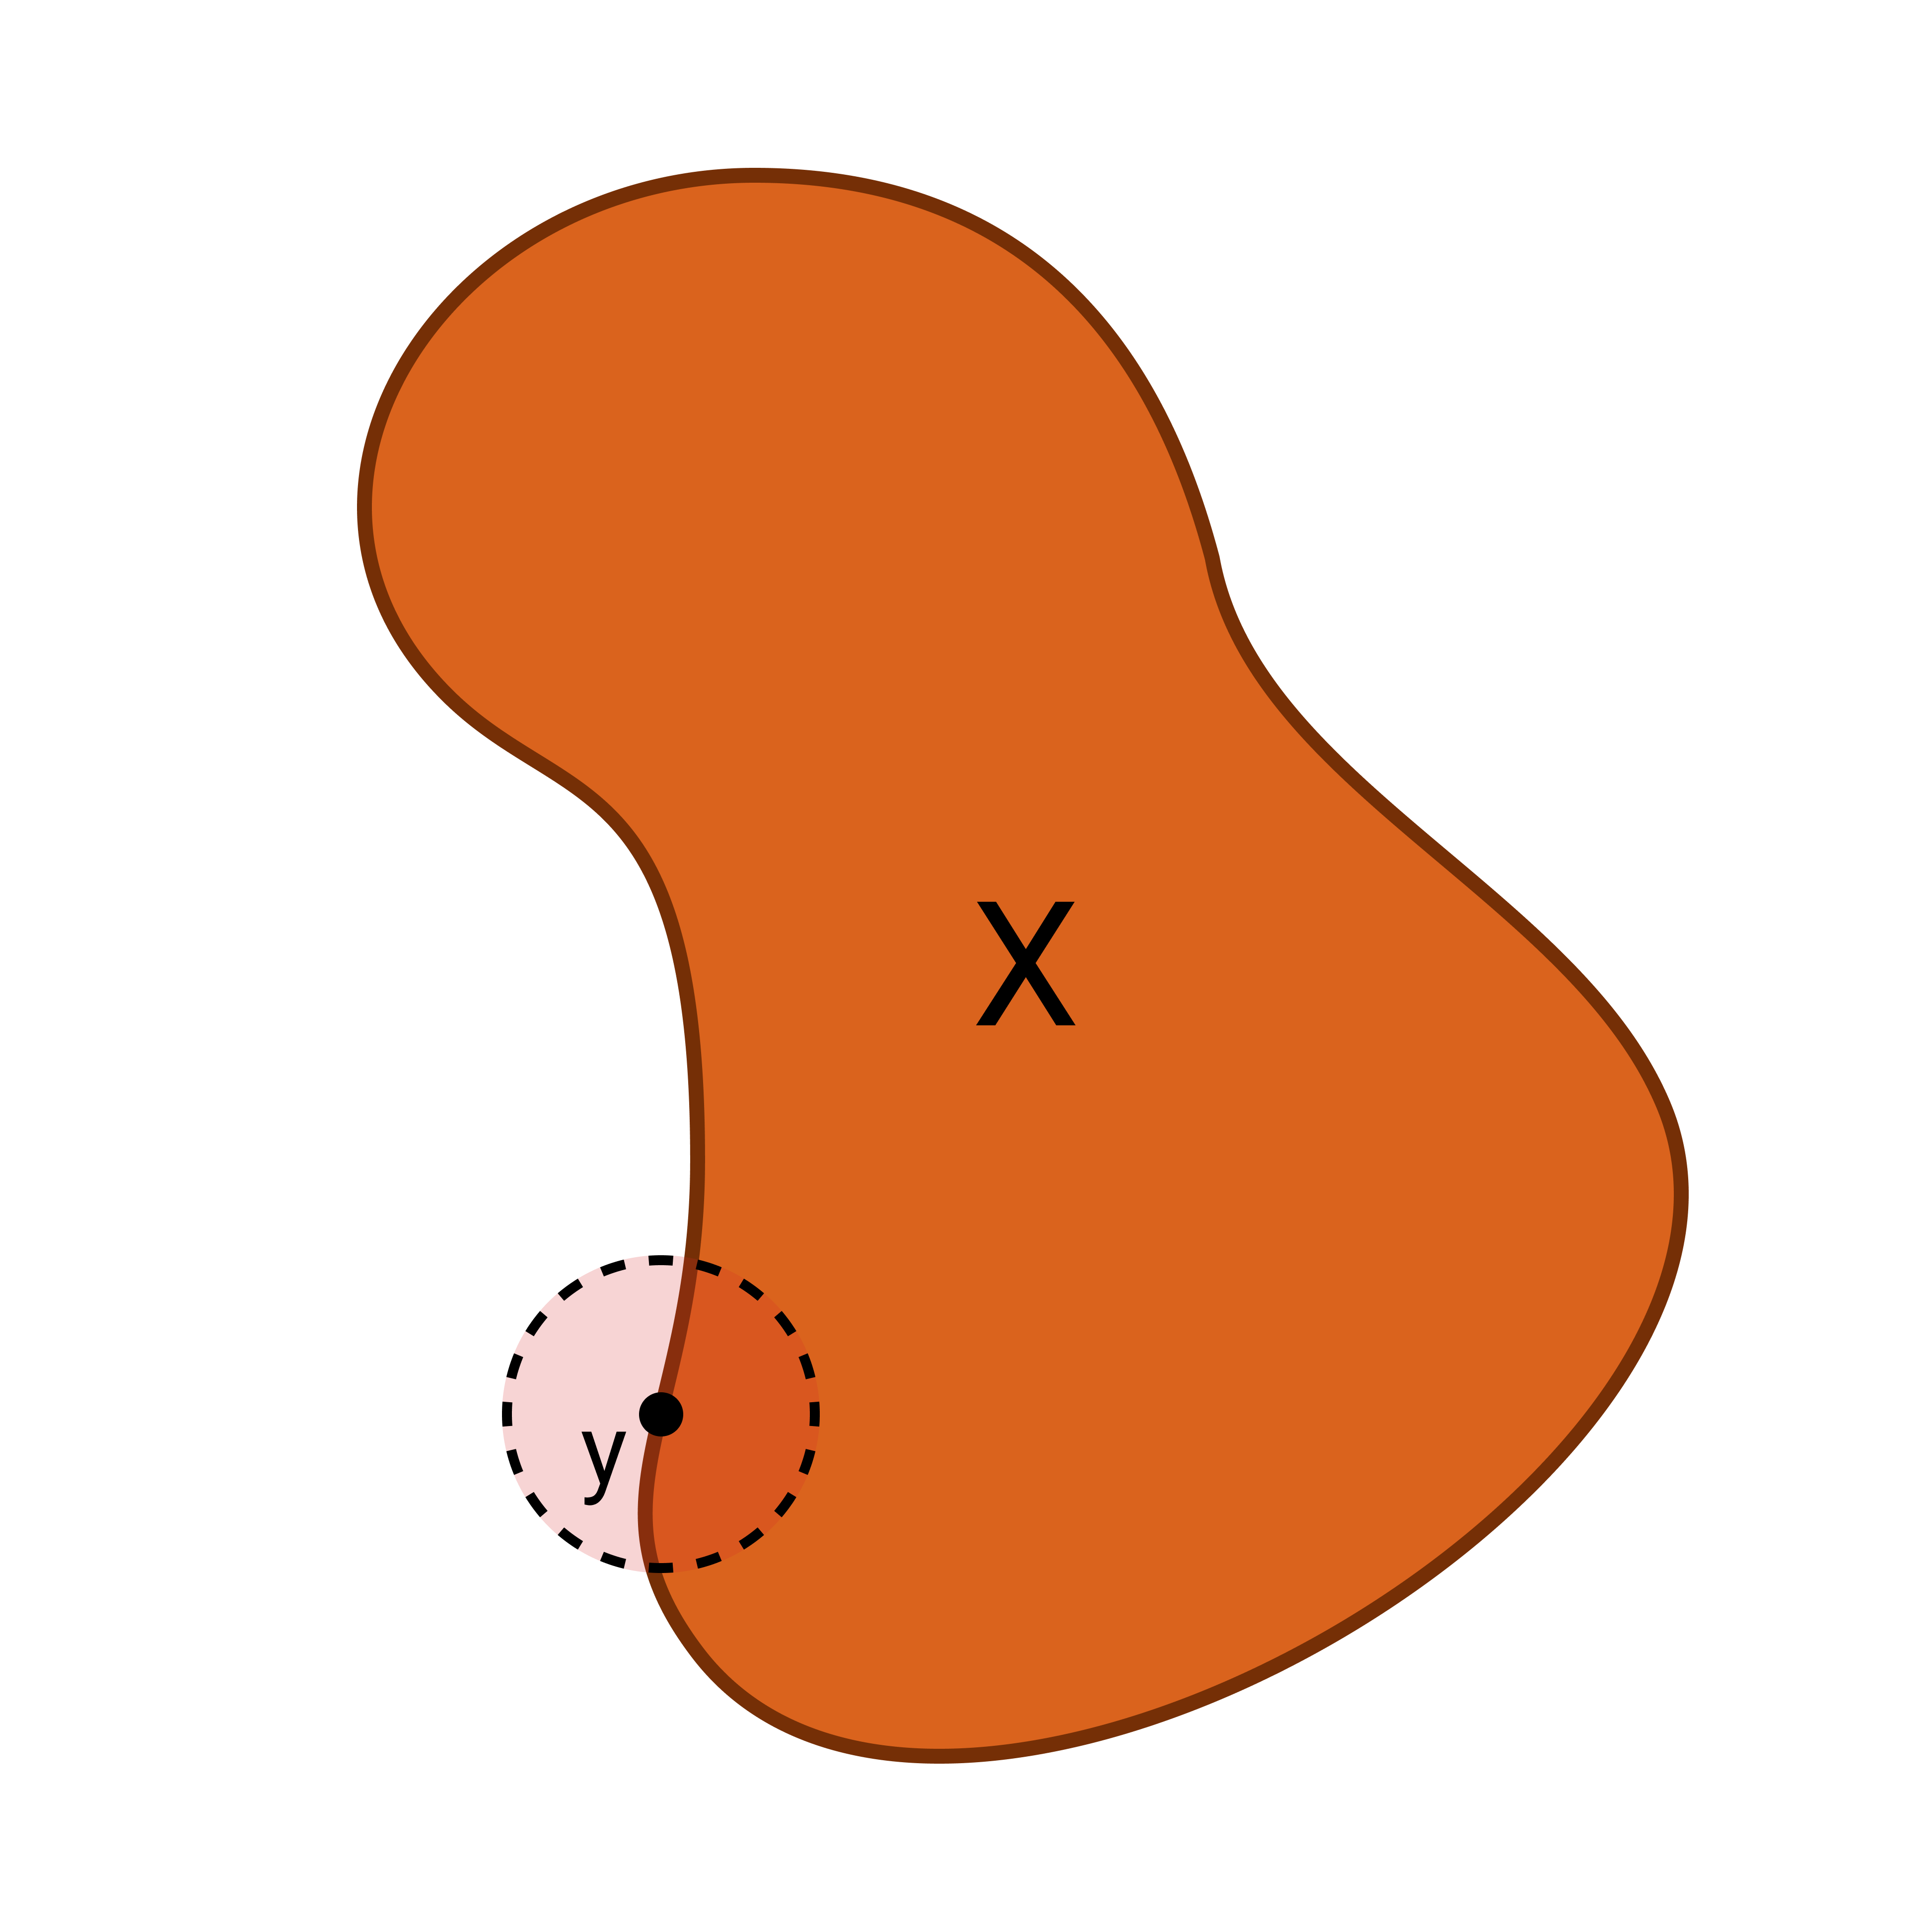
\includegraphics[width=0.3\textwidth]{section3/3.1/boundary.png}
	\end{center}
	\caption{Boundary point $y$ on a subset $X$.}
	\label{sect3:boundary}
\end{figure}
    
\subsubsection{Closure}
    
\begin{definition}
	The closure of a subset $X$, denoted $kX$, is the union of $X$ with the set of all its limit points. A point is a limit point of a subset $X$ of a topological space $(W, T)$ if each neighborhood of $x$ contains at least a point of $X$ different from $x$. \cite{Requicha1978MathematicalFO}
\end{definition}
    
\begin{figure}[ht]
	\begin{center}
		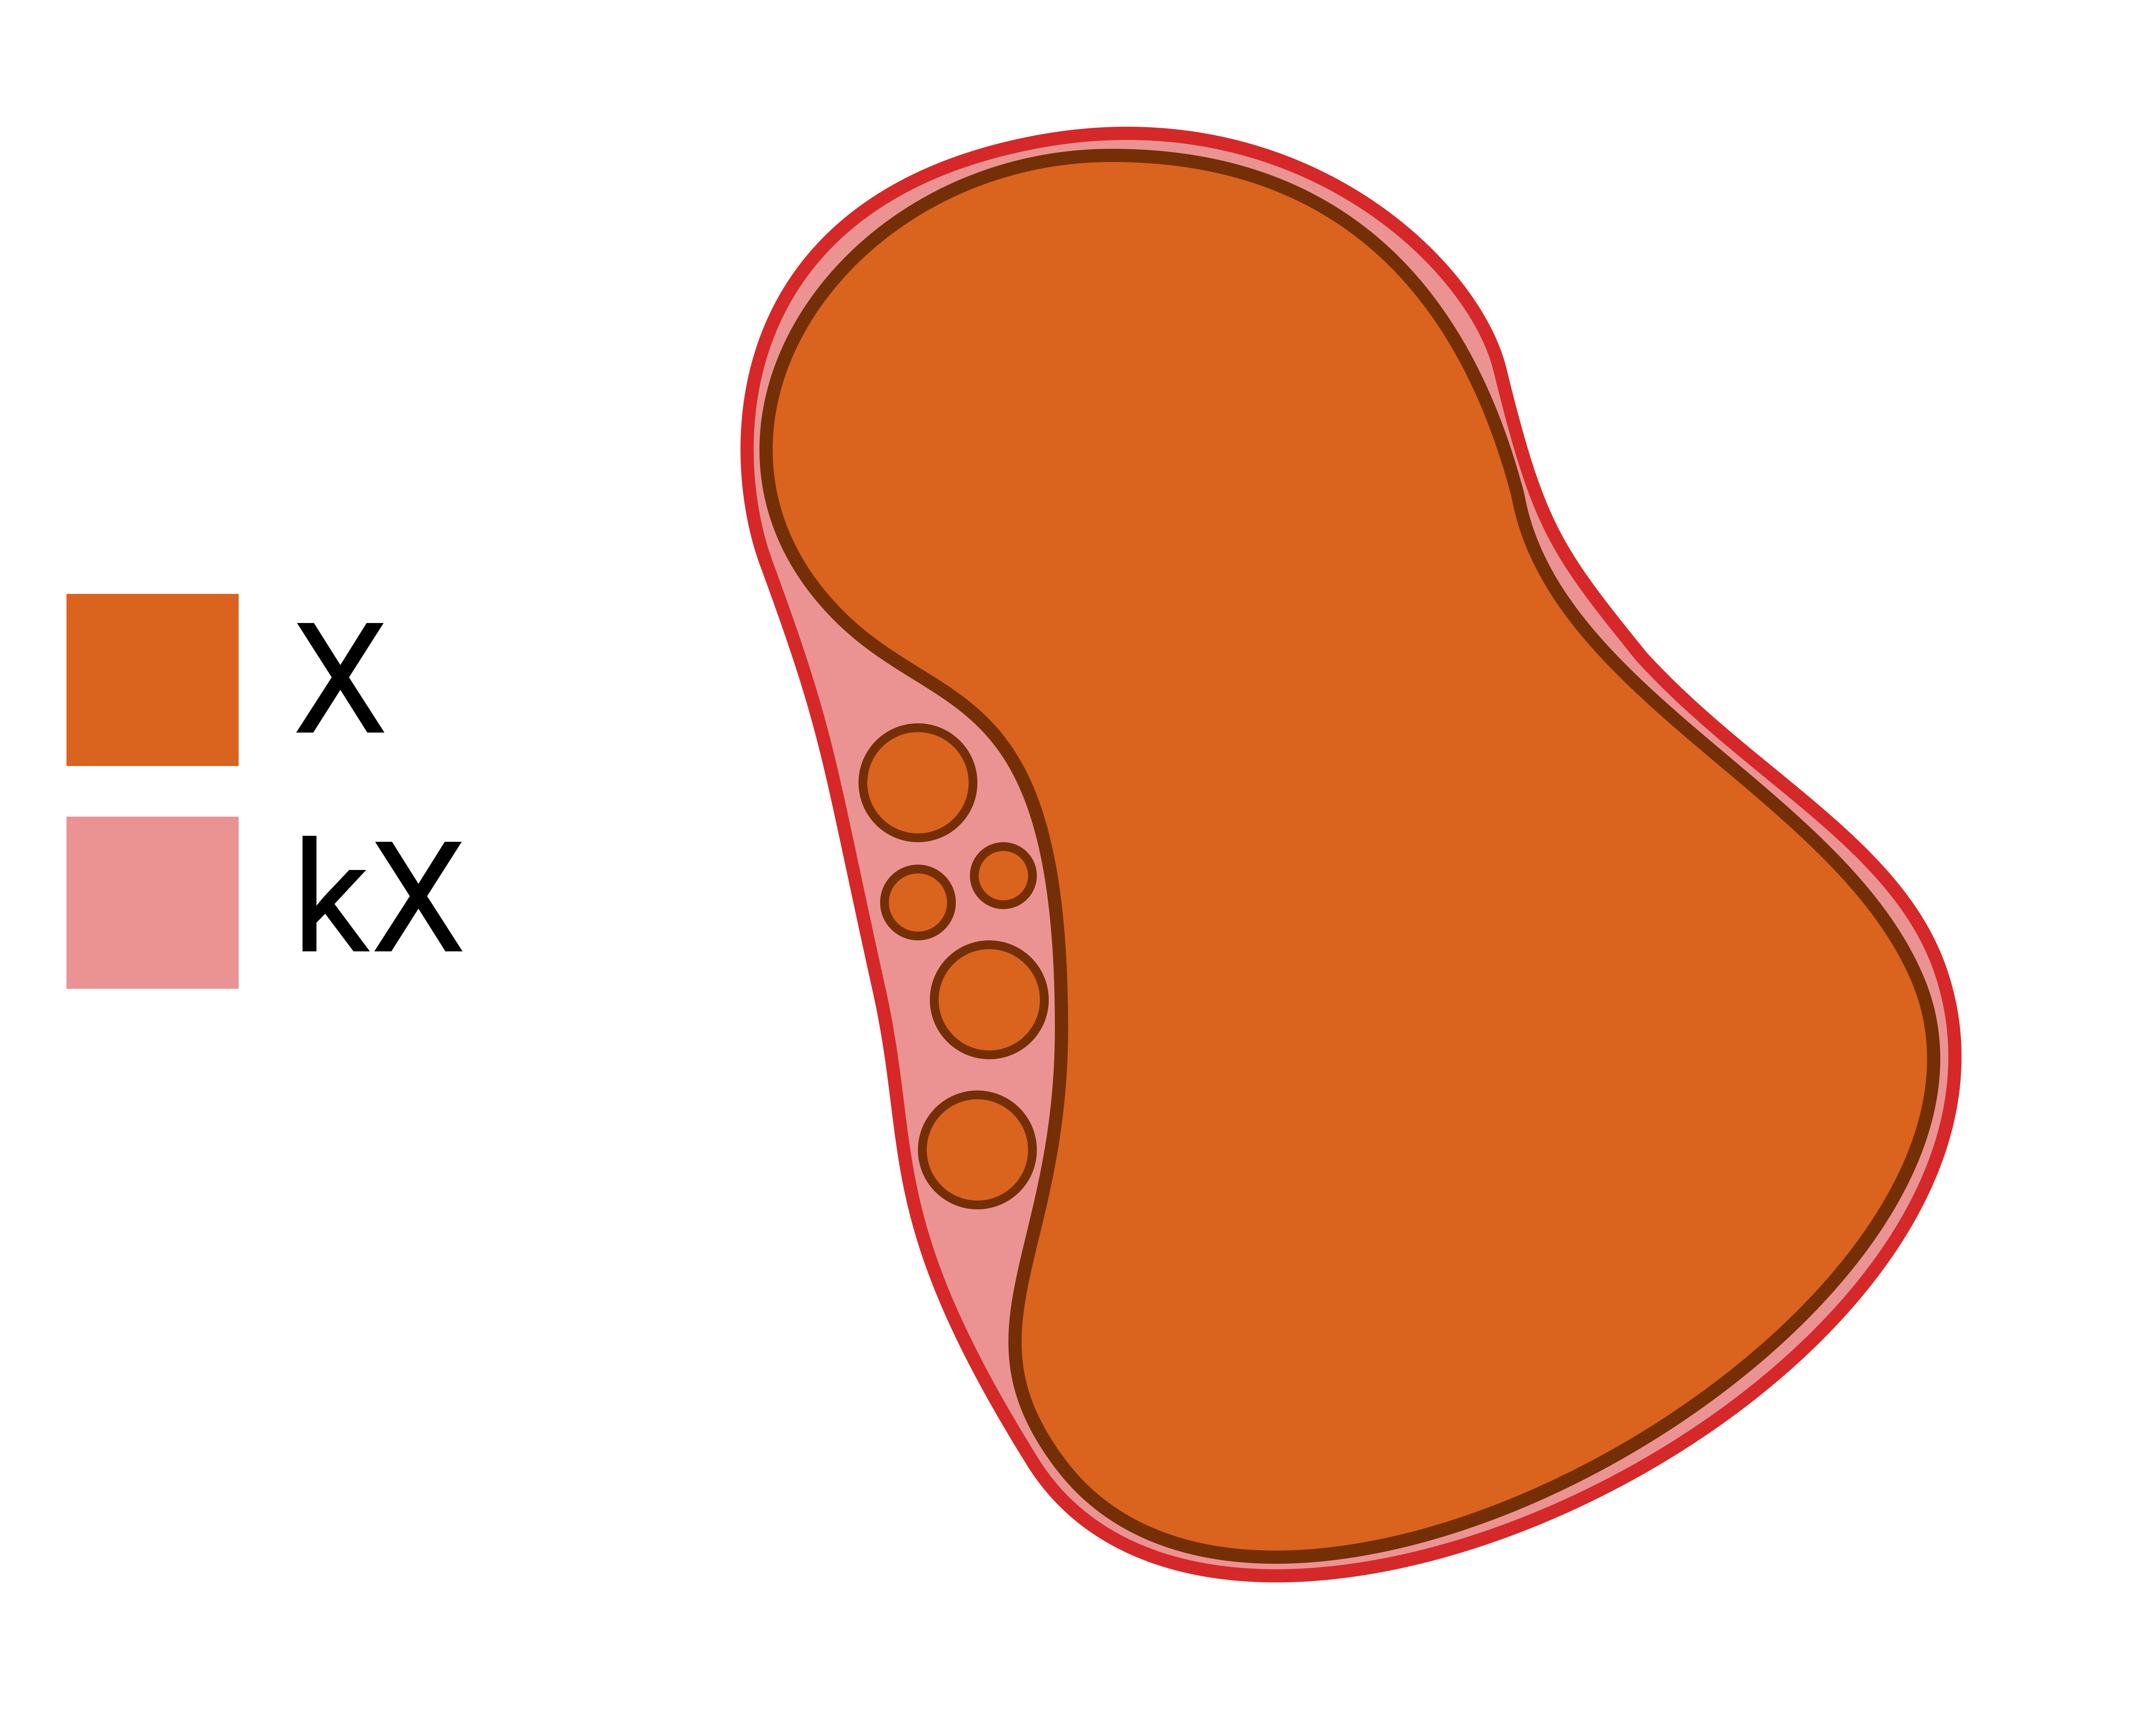
\includegraphics[width=0.3\textwidth]{section3/3.1/closure.png}
	\end{center}
	\caption{Closure $kX$ of a subset $X$.}
	\label{sect3:closure}
\end{figure}
    
\subsubsection{Regularity}
    
\begin{definition}[Regularity]
	The regularity of a subset $X$ of $W$, denoted $rX$, is the set of $rX = kiX$. \cite{mansfield_1987}
\end{definition}
\begin{definition}[Regular Set]
	A set $X$ is regular if $X = rX$, i.e. if $X = kiX$. \cite{mansfield_1987}
\end{definition}
    
\begin{definition}[Regularized Set Operators]
	The regularized union, intersection, difference and complement are defined per:
	\begin{align*} 
		X \cup^* Y   & = r(X \cup Y)    \\
		X \cap^* Y   & = r(X \cap Y)    \\
		X \ominus^*Y & = r(X \ominus Y) \\
		c{^x}X       & = rcX            
	\end{align*}
\end{definition}
    
\begin{figure}[ht]
	\begin{center}
		\includegraphics[width=0.8\textwidth]{section3/3.1/regularization.png}
	\end{center}
	\caption{Normal polygon intersection versus regularized intersection.}
	\label{sect3:regularization}
\end{figure}

\subsubsection{Membership Classification Function}
The membership classification function allows to segment a candidate set into three subsets which are the "inside", "outside", and "on the" of the reference set. Here, we will abstractly define what membership classification before moving to the practical implementations and implications of the more specific ray classification.
This theory depends heavily on the previously defined notions of interior, closure, boundary, and regularity. For a brief recapitulation, a point $p$ is an element of the interior of a set $X$, denoted $iX$, if there exists a neighborhood of $p$ that is contained in $X$; $p$ is an element of the closure of $X$, $kX$, if every neighborhood of $p$ contains a point of $X$; $p$ is an element of the boundary of $X$, $bX$, if $p$ is an element of both $kX$ and $k(cX)$, where $c$ denotes the complement. A set is said to be regular if $X = kiX$.

The membership classification function works on a pair of point sets:

\begin{conditions}
	S     &  The regular reference set in a subspace $W$. \\
	X     &  The candidate regular set $X$, classified with respect to $S$, in a subspace $W'$ of $W$. \\
\end{conditions}

Primed symbols will be used	in order to denote operations on the subspace $W'$ while normal symbols will be used to denote the subspace $W$: see table \ref{table:notations}.
 
\begin{table}
	\caption{Notation}
	\label{table:notations}
	\begin{tabularx}{\textwidth}{p{0.22\textwidth}X}
		\toprule
		$E^n$                                        & Euclidean n-space                                   \\
		$\emptyset$                                  & Empty Set                                           \\
		$W$                                          & Reference Set Universe                              \\
		$W'$                                         & Candidate Set Universe                              \\
		$\cup, \cap, \ominus, c$                     & Set Operators                                       \\
		$\cup^*, \cap^*, \ominus^*, c^*$             & Regularized Set Operators in $W$                    \\
		$\cup^{*'}, \cap^{*'}, \ominus^{*'}, c^{*'}$ & Regularized Set Operators in $W'$                   \\
		$i, b, k, r$                                 & interior, boundary, closure, and regularity in $W$  \\
		$i', b', k', r'$                             & interior, boundary, closure, and regularity in $W'$ \\
		\bottomrule
	\end{tabularx}
\end{table}

\begin{definition}
	The membership classification function, $M[]$ is defined as follows:
	\begin{equation}
		M[X, S] = (XinS, XonS, XoutS).
	\end{equation}
	where
	\begin{align*}
		XinS  & = X \cap^{*'} iS \\
		XonS  & = X \cap^{*'} bS \\
		XoutS & = X \cap^{*'} cS 
	\end{align*}
\end{definition}

The results obtained from this classification ($XinS, XonS, XoutS$) are the regular portions of the candidate set, $X$, in the interior, boundary, and the exterior of the reference set $W$: see figure \ref{sect3:membership_classification}.
The classification results also reflect a few properties. The produced results are a quasi-disjoint decomposition of the candidate; therefore:
\begin{equation}
	X = XinS \cup XonS \cup XoutS
\end{equation}
and for "almost" all points in the subset:
\begin{align*}
	XinS \cap XonS  & = \emptyset \\
	XonS \cap XoutS & = \emptyset \\
	XinS \cap XoutS & = \emptyset \\
\end{align*}
We say almost since the subsets are generally not disjoint in the conventional sense. (e.g. in figure \ref{sec3.2:fig2} $XinS$ and $XonS$ share a boundary point).



\begin{figure}[ht]
	\begin{center}
		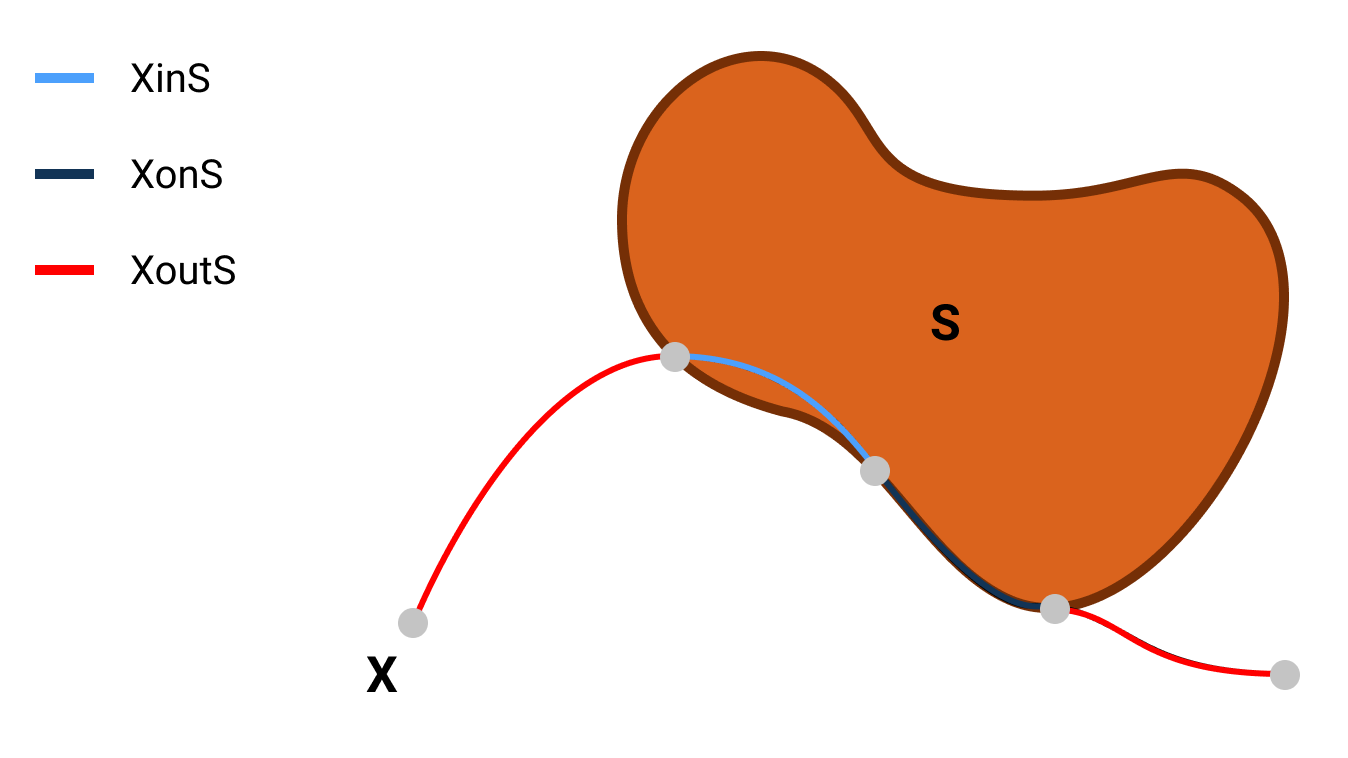
\includegraphics[width=0.5\textwidth]{section3/3.2/membership_classification.png}
	\end{center}
	\caption{Membership classification function.}
	\label{sect3:membership_classification}
\end{figure}

\subsubsection{Classification by constructive geometry}

Constructive geometry representations are binary trees whose nonterminal nodes designate regularized set operators and whose terminal nodes designate primitives.  We refer to the specific case of constructive geometry in $E^3$ where regularized compositions are constructed of solid primitives as Constructive Solid Geometry. Regular sets are closed under the regularized set operators thus a class of regular sets can be represented constructively as a combination of other more simple (regular) sets.

For example, as illustrated in Fig. \ref{sect3:halfplane-csg}, if the universe $W$ is in $E^2$ and we select the class of closed half-planes as our primitives, we could construct any regular set in $E^2$ given that it is bounded by a finite number of straight line segments.

\begin{figure}[ht]
	\begin{center}
		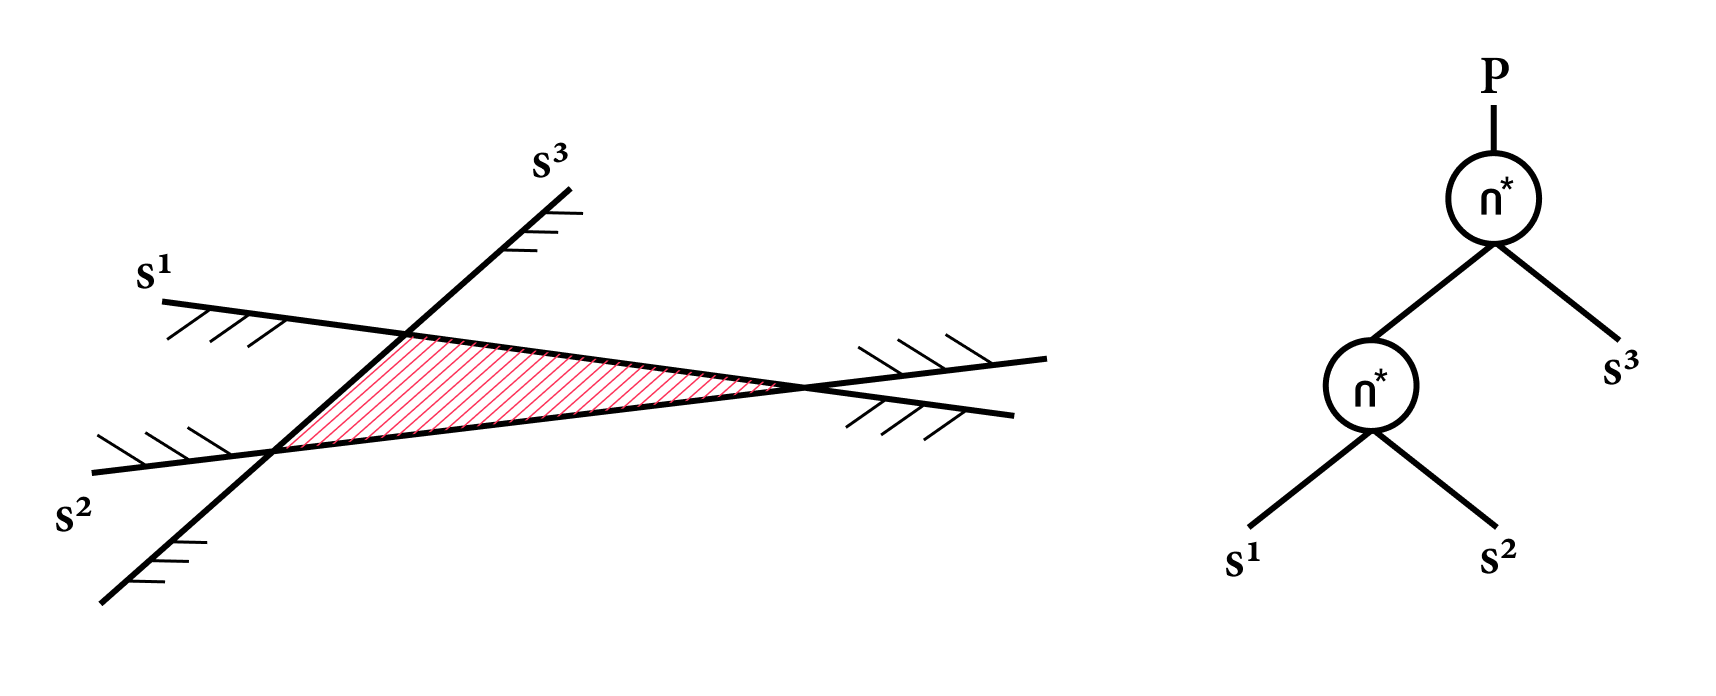
\includegraphics[width=0.8\textwidth]{section3/3.2/halfplane-csg.png}
	\end{center}
	\caption{A constructive representation of a polygon P using half-planes. The tree on the right is the constructive geometry representation.}
	\label{sect3:halfplane-csg}
\end{figure}

We choose to define the constructively represented regular sets using the divide-and-conquer paradigm as it is a natural approach to to compute the value of such a function. Therefore, when a regular set $S$ is not a primitive, a nonterminal node, we convert the problem of evaluating the function $f(S)$ into two simpler instance of $f$ evaluation followed by a combine, $g$, step. When $S$ is a primitive, a terminal node, the problem can no longer be divided and an evaluator, e-$f$, is used. We can now consider the general algorithm for evaluation $M[]$ when the reference set $S$ is represented constructively.

\begin{align}
	M[X,S]= 
	\begin{cases}
	\text{e-}M(X, S),                                                        & \text{if } S \subset A \\
	g(M[X, \text{l-subtree}(S)], M[X, \text{r-subtree}(S)], \text{root}(S)), & \text{otherwise}       
	\end{cases}
\end{align}

where

\begin{conditions}
	\text{e-}M     	  &  The primitive evaluation function. \\
	A     			  	  &  The set of all allowed primitives. \\
	g     				  &  The combine function. \\
	\text{l-subtree}     &  The left subtree. \\
	\text{r-subtree}     &  The right subtree. \\
	\text{root}     	  &  The operation type. \footnotemark \\
\end{conditions}
\footnotetext{The current node always contains the operation.}

To customize this general definition to be used in a specific domain, one must design the primitive classification procedure, e-$M$, and the combine procedure, $g$. We have already defined our primitive classification procedure in section \ref{section:ray-intersection}. The combine procedure is discussed thoroughly in the next section.

\subsection{Ray classification}

Given a ray and a solid composition tree, our procedure classifies the ray with respect to the solid and returns the classification to the caller. As previously defined, the classification of a ray with respect to a solid is the information describing the closest and furthest ray-solid intersection, $[in, out]$. The procedure starts at the top of the solid composition tree, recursively descends to the terminal nodes, classifies the ray with respect to the primitives, and then returns the tree combining the classifications of the left and right subtrees. As illustrated in \ref{ray-classification:boolean_algebra}, combining classifications is a matter of boolean algebra. \cite{ROTH1982109}

\begin{table}[h]
	\centering
	\label{ray-classification:boolean_algebra}
	\begin{tabular}{||c c c c||} 
		\hline
		Set Operator & Left Solid & Right Solid  & Composite \\ [0.5ex] 
		\hline\hline
		$\cup$    & IN & IN & IN  \\
		    	  & IN & OUT & IN  \\
		    	  & OUT & IN & IN  \\
		 	   	  & OUT & OUT & OUT  \\
		\\
		$\cap$    & IN & IN & IN  \\
		    	  & IN & OUT & OUT  \\
		    	  & OUT & IN & OUT  \\
		 	   	  & OUT & OUT & OUT  \\
		\\
		$\ominus$ & IN & IN & OUT  \\
		    	  & IN & OUT & IN  \\
		    	  & OUT & IN & OUT  \\
		 	   	  & OUT & OUT & OUT  \\		 	   	
		\hline
	\end{tabular}
\end{table}


\section{Optimization}

This section discusses criteria that are used to evaluate the
research results. Make sure your results can be used to published
research results, i.e., to the already known state-of-the-art.

(target size: 5-10 pages)

\section{Evaluation of the results}

Summarize the main aspects and results of the research
project. Provide an answer to the research questions stated earlier.

(target size: 1/2 page)

\section{Conclusion}

\newpage
%\bibliographystyle{unsrt}
%\bibliography{bsc-sample}
\printbibliography

\end{document}